\documentclass[journal, draftclsnofoot]{./styles/IEEEtran}
\usepackage{cite}
\usepackage{amsmath}

\ifCLASSINFOpdf
  \usepackage[pdftex]{graphicx}
  % declare the path(s) where your graphic files are
  \graphicspath{{../pdf/}{../jpg/}}
  \DeclareGraphicsExtensions{.pdf,.jpg,.png}
\fi

\usepackage{stfloats}
\fnbelowfloat

\usepackage{hyperref}

% correct bad hyphenation here
\hyphenation{}



\begin{document}

\title{Subreddit Recommendation Engine}
\author{Benjamin~Geiger and~Andrew~Price}
\date{6 May 2013}



% make the title area
\maketitle

\begin{abstract}
\end{abstract}

\section{Introduction}


\subsection{reddit And Its Organization}

reddit\footnote{``Remember: ``reddit'' is always
lowercase.''\cite{reddit-thealien}} is a link aggregation system with
community features.

reddit comprises numerous individual aggregators, known as
``subreddits'', each dedicated to a subject. Subreddits are
traditionally prefixed with ``\texttt{/r/}'', due to post syntax.  These
subjects include topics as wide as individual celebrities
(\href{http://reddit.com/r/JenniferLawrence}{\texttt{/r/JenniferLawrence}}),
specific genres of music
(\href{http://reddit.com/r/early2000sjams}{\texttt{/r/early2000sjams}}),
cities (\href{http://reddit.com/r/Tampa}{\texttt{/r/Tampa}}),
universities (\href{http://reddit.com/r/USF}{\texttt{/r/USF}}), hobbies
(\href{http://reddit.com/r/photography}{\texttt{/r/photography}}), and
research subjects
(\href{http://reddit.com/r/MachineLearning}{\texttt{/r/MachineLearning}}).

Users, or ``redditors'', submit links to external resources, or written
messages or questions, into these subreddits. Once submissions are
posted, redditors are able to comment on the submissions. It is expected
that submissions to a subreddit are related to the topic of that
subreddit; an individual redditor is able to post or comment in many
subreddits (see figure \ref{fig:reddit}).

\begin{figure*}[!t]
\centering
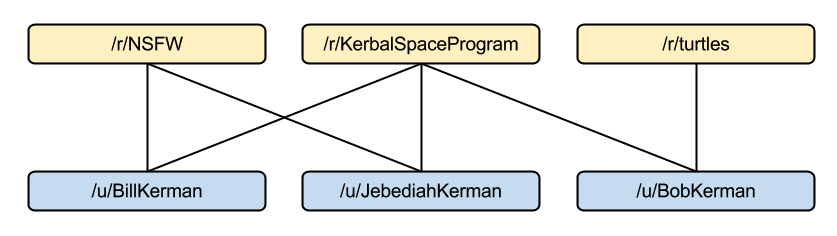
\includegraphics[width=\linewidth]{reddit.png}
\caption{Relationship between redditors (blue) and subreddits (yellow).}
\label{fig:reddit}
\end{figure*}

The primary feature of reddit is the voting system. Redditors are able
to vote to promote or suppress individual submissions or comments; a
submission receives mostly ``upvotes'' (votes to promote) will be more
favorably presented to those reading the subreddit, while a submission
that primarily receives ``downvotes'' (votes to suppress) will appear
further down the list. Likewise, comments that are mostly ``upvoted''
are presented earlier in the list of comments, where more readers are
likely to see them, while comments that are mostly ``downvoted'' are
presented further down the list; comments that receive many more
downvotes than upvotes are hidden by default, and must be explicitly
shown by the user (this is often the case for abusive or irrelevant
comments). Submissions that are irrelevant to the topic of the subreddit
are generally downvoted, encouraging the subreddit to remain on topic.

Each redditor has two ``karma'' scores, one for links and one for
comments. Each karma score is, approximately, the total of the upvotes
and downvotes given to that redditor's submissions or comments
respectively\footnote{Submissions that are not links are not counted
toward the user's link karma. Also, several heuristics are in place to
avoid rewarding fraudulent voting.}. As the name implies, users with
higher karma are generally seen as prominent members of the community,
while those with lower (or negative) karma have lower status.

In addition, each redditor is `subscribed' to several subreddits,
indicating that that redditor is interested in the topic of that
subreddit and wishes to see submissions posted therein. When
a redditor visits reddit, the `front page' shows the highest-voted
submissions from that redditor's subscribed subreddits; when someone who
is not a registered redditor visits reddit, the front page behaves as
though that person is subscribed to a collection of ``default
subreddits''\footnote{The current default subreddits, as of 4 May 2013,
are
\href{http://reddit.com/r/AdviceAnimals/}{\texttt{/r/AdviceAnimals}},
\href{http://reddit.com/r/announcements/}{\texttt{/r/announcements}},
\href{http://reddit.com/r/AskReddit/}{\texttt{/r/AskReddit}},
\href{http://reddit.com/r/atheism/}{\texttt{/r/atheism}},
\href{http://reddit.com/r/aww/}{\texttt{/r/aww}},
\href{http://reddit.com/r/bestof/}{\texttt{/r/bestof}},
\href{http://reddit.com/r/blog/}{\texttt{/r/blog}},
\href{http://reddit.com/r/funny/}{\texttt{/r/funny}},
\href{http://reddit.com/r/gaming/}{\texttt{/r/gaming}},
\href{http://reddit.com/r/IAmA/}{\texttt{/r/IAmA}},
\href{http://reddit.com/r/movies/}{\texttt{/r/movies}},
\href{http://reddit.com/r/Music/}{\texttt{/r/Music}},
\href{http://reddit.com/r/news/}{\texttt{/r/news}},
\href{http://reddit.com/r/pics/}{\texttt{/r/pics}},
\href{http://reddit.com/r/politics/}{\texttt{/r/politics}},
\href{http://reddit.com/r/science/}{\texttt{/r/science}},
\href{http://reddit.com/r/technology/}{\texttt{/r/technology}},
\href{http://reddit.com/r/todayilearned/}{\texttt{/r/todayilearned}},
\href{http://reddit.com/r/videos/}{\texttt{/r/videos}},
\href{http://reddit.com/r/worldnews/}{\texttt{/r/worldnews}},
and \href{http://reddit.com/r/WTF/}{\texttt{/r/WTF}}.
}. New users are subscribed to these subreddits automatically when their
accounts are created.

Intuitively, the topics covered by subreddits often follow a
hierarchical structure, as represented in figure \ref{fig:overlap}(a);
there will often be a single large subreddit that covers a wide topic
(such as all Ford vehicles), with smaller subreddits serving to host
more in-depth discussion of a narrower topic (such as Ford Mustangs).
However, interests also follow a pattern closer to figure
\ref{fig:overlap}(b), where the topic of a small subreddit is well
expressed as the combination of the topics of two larger subreddits.

\begin{figure*}[!t]
\centering
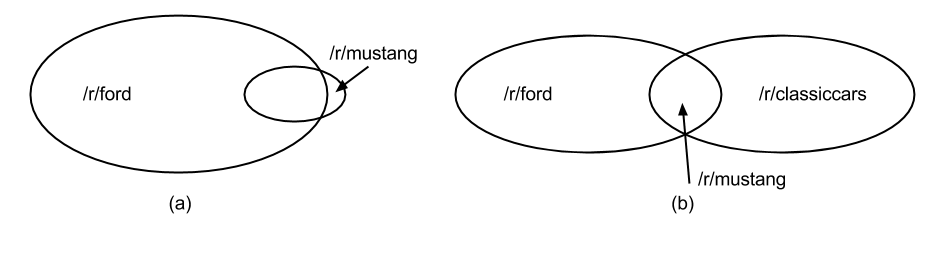
\includegraphics[width=\linewidth]{overlap.png}
\caption{Relationship between the topics of example subreddits.}
\label{fig:overlap}
\end{figure*}

\section{Motivation}

There are at least 239,434 subreddits as of 4 May 2013\cite{metareddit};
of those, only 5,326 are considered `active' (having 5 or more
submissions or comments in a day)\cite{reddit-aboutreddit}. Smaller
subreddits are often smaller simply because few people realize they
exist; having found the larger subreddits, they stop looking for smaller
subreddits that might better reflect their interests. This becomes a
self-fulfilling prophecy, as the smaller subreddits become less
interesting due to a lack of submissions.

\section{Methodology}

\subsection{Algorithm Development}

When developing our system, we started with three assumptions:

\begin{enumerate}

\item Links and comments with high scores are those that reflect the
topic of the subreddit they're posted in.

\item People who visit a subreddit tend to share a particular interest,
as specified in the topic of the subreddit.

\item Interests tend to not be independent; people who share one
interest are likely to share other related interests.

\end{enumerate}

This leads us to the primary question: How do we determine how much
overlap of interest exists between the topics of any two subreddits?

The na\"i{}ve approach is to determine the overlap in the readership
between the subreddits. However, this fails due to privacy issues:
reddit does not reveal the subreddits a redditor is subscribed to to
anyone other than that redditor. Another similar approach is to see
which links and comments each redditor has upvoted and downvoted, but
that fails for the same reason: individual votes are not revealed to
anyone other than the voter.

We instead had to find some indicator of user interest in a subreddit,
and settled on user posts. While a small fraction of the subscribers to
a subreddit ever post, the proportion that posts could be assumed to be
representative, absent other data. The posts and comments in most
subreddits are visible to the public.

One issue to consider, however, is that of `alts' or `throwaways'.
It is widely acceptable within the reddit community to have multiple
accounts, often to prevent intermingling of so-called `NSFW' (not safe
for work) activity with more `respectable' posts. Some of these accounts
exist only for a single post, and are referred to as `throwaways' (as
they are `thrown away' after that post). We decided that this was
negligible, as we assumed that most redditors are unlikely to use
different accounts for closely related subreddits.

\subsection{Algorithm Specification}

We decided to represent reddit as a weighted digraph $G = (V, E)$, with
each vertex $v \in V$ representing a subreddit and each edge $(v_1, v_2,
w_{v_1v_2}) \in E$ representing the likelihood $w_{v_1v_2}$ that a user
interested in the topic of $v_1$ will also be interested in the topic of
$v_2$. This graph is complete, as shown in figure \ref{fig:graph}; edges
between independent subreddits have a weight of 0.

\begin{figure}[!t]
\centering
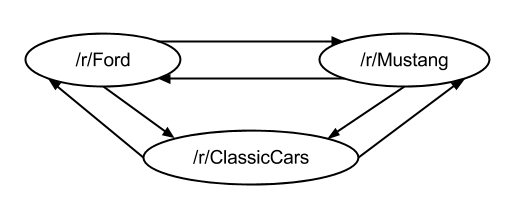
\includegraphics[width=\columnwidth]{graph.png}
\caption{Example of subreddit digraph.}
\label{fig:graph}
\end{figure}

The weight of an edge, $w_{v_1v_2}$, is the sum of several subscores:

\begin{align*}
w_{v_1v_2} &= \sum_{r \in (R(v_1) \cap R(v_2))} \left[ w_L L(r, v_2) + w_C C(r,
v_2) \right]\\
&+ w_X \sum_{s \in (S(v_1) \cap S(v_2)), K(s, v_1) > 0} K(s, v_2)
\end{align*}

where $L(r, v)$ is the sum of the scores for submissions by redditor $r$
in subreddit $v$, $C(r, v)$ is the same \textit{mutatis mutandis} for
comments instead of submissions, and $K(s, v)$ is the score of
submission $s$ in subreddit $v$. (Properly, a single submission is
defined as being part of its subreddit, and therefore can only exist in
one subreddit, but for the purpose of this algorithm, two submissions
are considered the same if they link to the same URL.)

As we are assumed to know our user's subscribed subreddits (or at the
very least, will be provided a set of subreddits with which to provide
recommendations), we can call that set of subreddits $S$ and construct a
secondary graph, $G' = (V \cup \{s'\}, E \cup E')$, in which $s$ is a
dummy starting node and $E' = (s, v, w_{sv})$ is a set of edges from $s$
to each node $v \in V\backslash S$, and $w_{sv} = \sum_{s' \in S}
w_{s'v}$.

The recommended subreddits are simply the subreddits $v \in V\backslash
S$ for which $w_{sv}$ is the greatest.

\section{Results}

\textit{todo: explain reddit api calls}

\textit{todo: explain data acquisition problems}

\textit{todo: give results from partial data}

\section{Conclusions}

\textit{todo: apologize for being a complete and utter fuckwit}




% Include all citations (because bibTeX is stupid)
\nocite{*}
\bibliographystyle{IEEEtran}
\bibliography{report}

% that's all folks
\end{document}


